\documentclass[sigconf]{acmart}

\usepackage[parfill]{parskip}
\usepackage{booktabs} % For formal tables
\usepackage{hyperref}


% Copyright
%\setcopyright{none}
%\setcopyright{acmcopyright}
\setcopyright{acmlicensed}
%\setcopyright{rightsretained}
%\setcopyright{usgov}
%\setcopyright{usgovmixed}
%\setcopyright{cagov}
%\setcopyright{cagovmixed}

% DOI
\acmDOI{http://dx.doi.org/10.1145/3055116.3055123}

% ISBN
\acmISBN{978-1-4503-4797-6/17/02}
\acmPrice{15.00}

%Conference
\acmConference[ICGJ 2017]{International Conference on Game Jams}{February 26 2017}{San Francisco, California USA} 
\acmYear{2017}
\copyrightyear{2017}


\begin{document}
	
\title{Major Tom}
\subtitle{Created in 48 hours for Global Game Jam 2017}

\author{Elliot Fiske}
\affiliation{%
  \institution{California Polytechnic State University}
  \streetaddress{4173 Acapulco Drive}
  \city{Campbell} 
  \state{California} 
}
\email{elliotfiske@gmail.com}

\author{Thomas Steinke}
\affiliation{%
  \institution{California Polytechnic State University}
  \streetaddress{3494 Kilo Avenue}
  \city{San Jose} 
  \state{California} 
}
\email{exyphnos@gmail.com}

\author{Alex Ling}
\affiliation{%
  \institution{California Polytechnic State University}
  \streetaddress{360 Cambridge St.}
  \city{San Francisco} 
  \state{California}}
\email{alex.ling.9495@gmail.com}

\author{Cory Slaught}
\affiliation{
  \institution{California Polytechnic State University}
  \streetaddress{27 Middle Ridge Ln.}
  \city{Rolling Hills} 
  \state{California}}
\email{coryslaught@gmail.com}

\begin{abstract}
In this paper, we describe our showcase submission --- the co-operative VR game Major Tom. We show how the constraints of a game jam led to a unique gameplay experience.
\end{abstract}

% We no longer use \terms command
%\terms{Theory}

\keywords{Game jam, local multiplayer, showcase, game development, videogames, Vive, virtual reality, Unity}


\maketitle

\section{Game Description}

\textit{Major Tom} is a two-player co-operative game for the HTC Vive. One player ("Major Tom", \textbf{\hyperref[fig:majortom]{Figure \ref*{fig:majortom}}}) wears the Vive headset and interacts with controls and objects in the ship. The other plaer ("Ground Control," \textbf{\hyperref[fig:groundcontrol]{Figure \ref*{fig:groundcontrol}}}) manages the control panel from outside virtual reality, and relays instructions and information to the player in virtual reality. The players must work together to operate the poorly-labeled spaceship and enter orbit.


\section{Gameplay}
The objective of \textit{Major Tom} is to start your spaceship's engines and ascend to 30,000 feet. Unfortunately, the spaceship's controls have no labels, so Major Tom must work closely with Ground Control to understand the state of the spaceship's engine, thrusters and brakes. Ground Control must keep the radio aligned with a frequency slider to hear voice instructions that are playing across the airwaves. Using these instructions, Ground Control must tell the player in VR to pull various levers or push buttons to try and get the spaceship off the ground.


\begin{figure*}[p]
	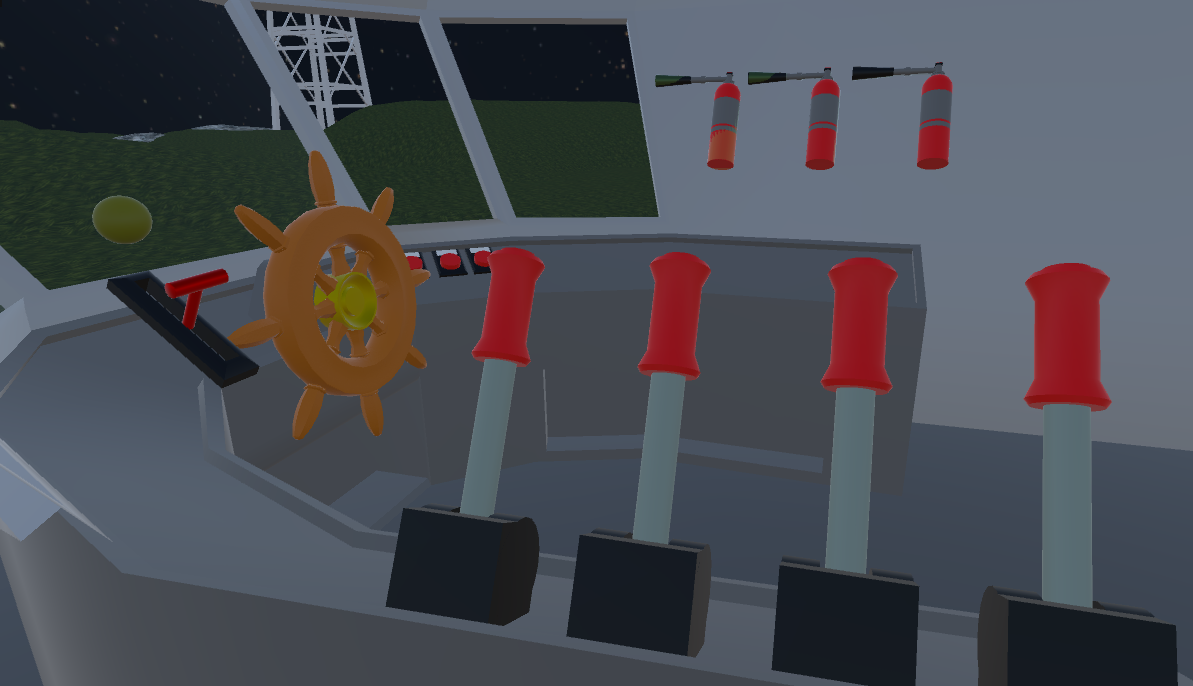
\includegraphics[width=6.5in]{MAJOR_TOM_VR}
	\caption{The "Major Tom" VR interface. You can see the steering wheel which adjusts the angle of the ship, as well as the various unlabeled buttons and levers. Players interact with the buttons, levers and fire extinguishers with the Vive controllers.}
	\label{fig:majortom}
\end{figure*}

\begin{figure*}[p]
	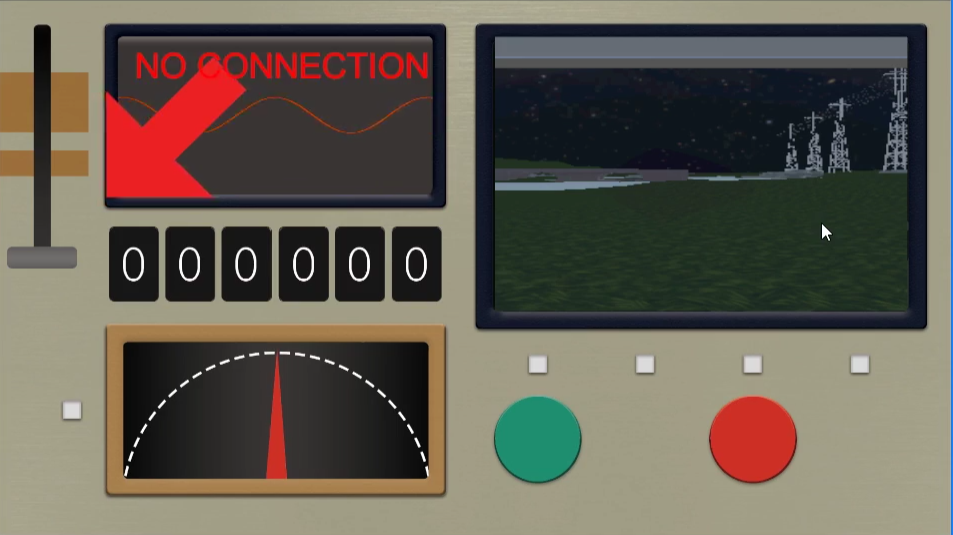
\includegraphics[width=6.5in]{MAJOR_TOM_GroundControl1}
	\caption{The "Ground Control" interface. In this view, the player \textit{not} in VR can see the view facing out the front of the spaceship, as well as some knobs and dials that will be used later in the game.}
	\label{fig:groundcontrol}
\end{figure*}

\section{Development}
The concept, design and all the assets for \textit{Major Tom} were created in 48 hours for the Global Game Jam. We used tools that we had experience with to accelerate the development process. We used Unity as the game engine, MODO 10 for modeling and textures, Photoshop for the UI assets, and Audacity to record and edit the voiceovers.

\subsection{Diversifiers}
The main idea for our game originated from one of the "diversifiers" for the Global Game Jam. In addition to the main theme, Global Game Jam provides a long list of optional diversifiers that jammers can use to challenge themselves, creating interesting design constraints or improving the accessibility of the game.

Although the diversifiers are optional to use, we've found that implementing them adds interesting depth, as you work around the constraint or use it for inspiration. In this case, the diverisifer we focused on was called "VRiends: Create a VR game where people inside VR and people outside VR have to work together." We took this basic idea and used it to drive the design of \textit{Major Tom} forward. We began with the idea that the player outside VR would have information necessary to the player inside VR, so they would need to communicate with each other to win the game. We drew inspiration from cooperative games like \textit{Spaceteam} and \textit{Keep Talking and Nobody Explodes}.

The diversifier also influenced the narrative of the game. We needed to justify why the spaceship would be missing labels, so we established that the player's space program is haphazard and dangerous, with references to previous failed missions and missing safety features in the spaceship.

To convey all this information, we decided we needed to record voiceovers. Fortunately, the venue of the Global Game Jam had soundproof booths for taking calls with customers. With the host company's permission, these became perfect sound recording studios to make our voiceovers.

To make a successful game in 48 hours, our team utilized available resources and worked \textit{with} design constraints rather than against them. Being flexible and willing to adjust your ideas to compromise with the vision of the team leads to an enjoyable, productive game jam.

\subsection{Development Achievements}
One of the main challenges was integrating the 2D "Ground Control" interface with the VR "Major Tom" interface. Several ideas were proposed, such as using two separate Unity projects connected via sockets. However, given the limited time frame of the jam, we came to a much more elegant solution. 

Unity lets you have multiple cameras in the scene, and allows you to selectively enable or disable certain categories of objects for each camera. We used two cameras to target each of the VR "eyes," and created a separate static camera that could only see the 2D user interface. This way, controlling the 2D "Ground Control" interface is as simple as starting the Unity project and using the interface on the host computer, while the other player is in VR.

Our solution was quick and effective, and let us drop in a cool extra feature for free. Since we already had multiple custom cameras rendering to different views, we added one more to create the "GoPro" effect in \textbf{\hyperref[fig:groundcontrol]{Figure \ref*{fig:groundcontrol}}}. The camera is affixed to the front of the spaceship, and renders to a texture that appears in the Ground Control interface, helping connect the Ground Control player to the action going on in VR.

\subsection{Development Strategy}
Our previous experience with game jams showed us the value of iterating quickly. Our general strategy for game jams is to create a playable prototype as fast as possible and to identify the "core fun" that we can expand into a full game. We continue to make as many playable prototypes as we can, refining the concept and adding fun details.

\section{Availability}
\textit{Major Tom} is available from its Global Game Jam 2017 submission page: \textbf{\href{http://globalgamejam.org/2017/games/major-tom}{http://globalgamejam.org/2017/games/major-tom}}. Its source code is available at \textbf{\href{https://github.com/epiphane/majortom}{https://github.com/epiphane/majortom}}.

Given the difficulty of running the game as it requires a Vive headset, you can watch a gameplay video at \textbf{\href{http://www.elliotfiske.com/majortom/}{http://www.elliotfiske.com/majortom/}}


\end{document}
